\documentclass[12pt, titlepage]{article}

\usepackage{booktabs}
\usepackage{tabularx}
\usepackage{hyperref}
\hypersetup{
    colorlinks,
    citecolor=black,
    filecolor=black,
    linkcolor=red,
    urlcolor=blue
}
\usepackage[round]{natbib}
\usepackage{graphicx}
\usepackage{subfig}

%% Comments

\usepackage{color}

\newif\ifcomments\commentstrue %displays comments
%\newif\ifcomments\commentsfalse %so that comments do not display

\ifcomments
\newcommand{\authornote}[3]{\textcolor{#1}{[#3 ---#2]}}
\newcommand{\todo}[1]{\textcolor{red}{[TODO: #1]}}
\else
\newcommand{\authornote}[3]{}
\newcommand{\todo}[1]{}
\fi

\newcommand{\wss}[1]{\authornote{blue}{SS}{#1}} 
\newcommand{\plt}[1]{\authornote{magenta}{TPLT}{#1}} %For explanation of the template
\newcommand{\an}[1]{\authornote{cyan}{Author}{#1}}

%% Common Parts

\newcommand{\progname}{ProgName} % PUT YOUR PROGRAM NAME HERE
\newcommand{\authname}{Team \#, Team Name
\\ Student 1 name
\\ Student 2 name
\\ Student 3 name
\\ Student 4 name} % AUTHOR NAMES                  

\usepackage{hyperref}
    \hypersetup{colorlinks=true, linkcolor=blue, citecolor=blue, filecolor=blue,
                urlcolor=blue, unicode=false}
    \urlstyle{same}
                                


\begin{document}

\title{Verification and Validation Report: \progname} 
\author{\authname}
\date{\today}
	
\maketitle

\pagenumbering{roman}

\section{Revision History}

\begin{tabularx}{\textwidth}{p{3cm}p{2cm}X}
\toprule {\bf Date} & {\bf Version} & {\bf Notes}\\
\midrule
2025-04-16 & Rev 1.0 & Initial Release\\
\bottomrule
\end{tabularx}

~\newpage

\section{Symbols, Abbreviations and Acronyms}

\renewcommand{\arraystretch}{1.2}
\begin{tabular}{l l} 
  \toprule		
  \textbf{symbol} & \textbf{description}\\
  \midrule 
  CSV & comma separated value \\
  FAST & Features from Accelerated Segment Test \\
  IFCS & \progname{} software\\
  T & Test\\
  \bottomrule
\end{tabular}\\


\newpage

\tableofcontents

\listoftables %if appropriate

\listoffigures %if appropriate

\newpage

\pagenumbering{arabic}

This document outlines the results of the system and unit tests for the \progname  $ $ software. The detaileds of the associated tests are outlined in the \href{https://github.com/KiranSingh15/CAS-741-Image-Correspondences/blob/main/docs/VnVPlan/VnVPlan.pdf}{\textbf{VnV Plan}}.
\section{Functional Requirements Evaluation}


\subsection{Feature Detection}
\paragraph{Image Smoother}

\begin{enumerate}
\item \hypertarget{STFR-IS-01}{\textbf{STFR-IS-01}} \\ \\ 
This test evaluates the capacity of the system to import generated ArUco marker imagery, convert the imagery to a greyscale format, perform Gaussian smoothing, and save both the greyscale and smoothed images using a kernel size of 5 and a standard deviation of 1.0. This test was manually initiated and executed via Pytest using the \href{https://github.com/KiranSingh15/CAS-741-Image-Correspondences/blob/main/src/tests/test_STFR-IS-01.py}{test\_STFR-IS-01.py} program. The test passed all checks and provides a \href{https://github.com/KiranSingh15/CAS-741-Image-Correspondences/blob/main/src/tests/Outputs/2025-04-13_12-19-08/summary.txt}{summary.txt} of the results under its timestamped \href{https://github.com/KiranSingh15/CAS-741-Image-Correspondences/tree/main/src/tests/Outputs/2025-04-13_12-19-08}{STFR-IS-01} output folder. \\ \\
\textit{Requirements Addressed:}
\begin{itemize}
\item R1 (Update Image Noise) 
\item R5 (Default Noise Suppression)
\item R9 (Perform Noise Reduction)
\end{itemize}

Figure \ref{fig-IS-AR} shows an example of the generated greyscale and smoothed imagery of the ArUco markers. All generated output imagery can be reviewed in the \href{https://github.com/KiranSingh15/CAS-741-Image-Correspondences/tree/main/src/tests/Outputs/2025-04-13_12-19-08}{STFR-IS-01} output folder.\\


\begin{figure}[h!]
  \centering
  \subfloat[Converted Greyscale Image \label{AR-GS}]{
  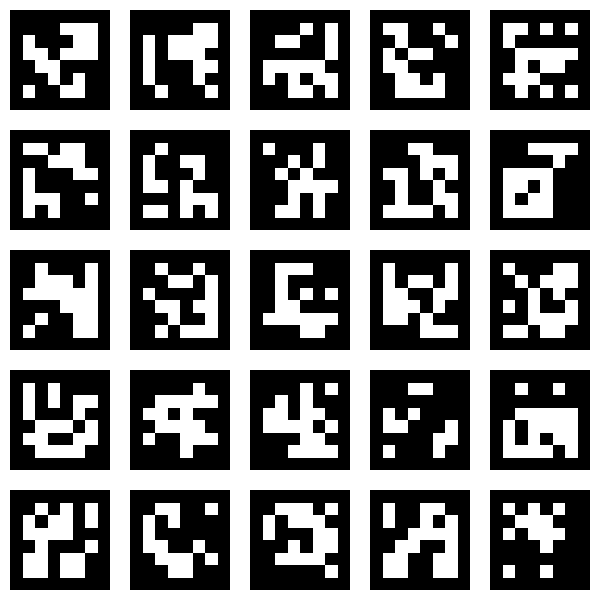
\includegraphics[width=0.45\linewidth]{images/gs_aruco_000.png}
  }
  \hfill
  \subfloat[Gaussian-Smoothed Image \label{AR-GK}]{
  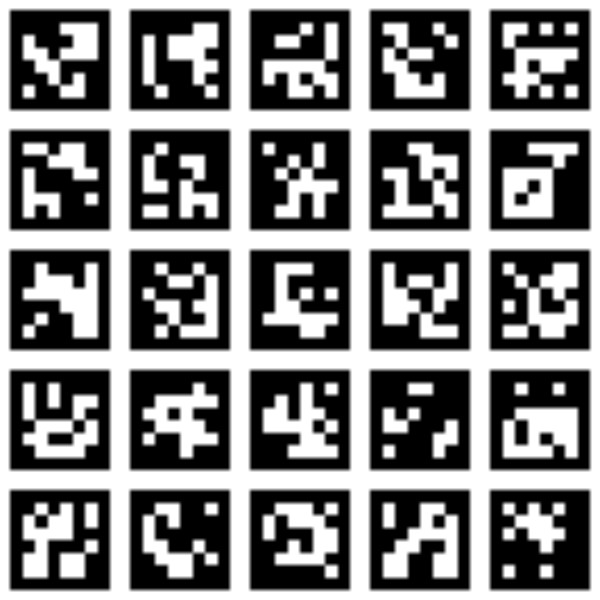
\includegraphics[width=0.45\linewidth]{images/aruco_000.png}
  }
  \caption{Outputs of the image smoothing procedure on an untransformed ArUco marker}
  \label{fig-IS-AR}
\end{figure}


As the results from processing a binary ArUco marker do not produce a distinct change in colour to the human eye, a second test was executed on the test imagery provided in the \href{https://github.com/KiranSingh15/CAS-741-Image-Correspondences/tree/main/src/tests/testImages/building}{testImages\textbackslash building} folder.

\begin{figure}[h!]
  \centering
  \subfloat[Building - RGB Input Image \label{UH-IN}]{
  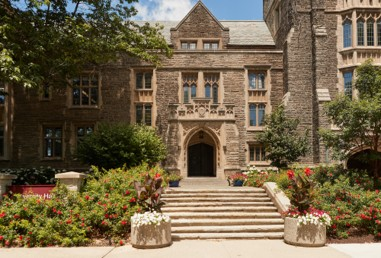
\includegraphics[width=0.45\linewidth]{images/UH_raw.jpg}
  }
  \hfill
  \subfloat[Building - Greyscale Image \label{UH-GS}]{
  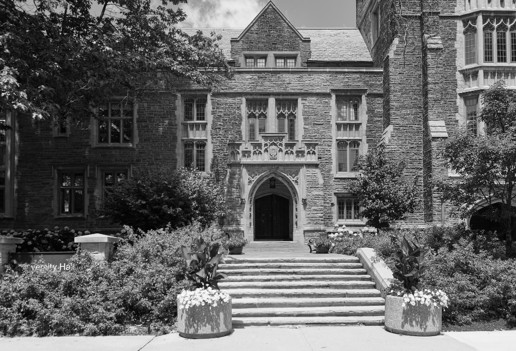
\includegraphics[width=0.45\linewidth]{images/UH_gs.jpg}
  }
  \hfill
  \subfloat[Building - Smoothed Image \label{UH-SM}]{
  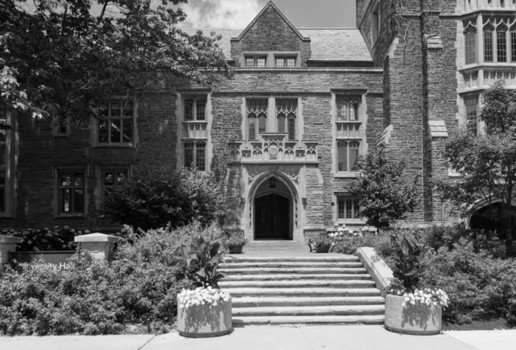
\includegraphics[width=0.45\linewidth]{images/UH_is.jpg}
  }
  \caption{Greyscale and noise-reduced images generated from the building dataset}
  \label{fig-building}
\end{figure}

\end{enumerate}

\newpage

\paragraph{Keypoint Detection}
\begin{enumerate}

\item \hypertarget{STFR-KP-01}{\textbf{STFR-KP-01}}\\
This test evaluates the capacity of the system to import smoothed ArUco marker imagery and identify keypoints through use of rotated-FAST methods. A pixel intensity threshold of 60 was set for this test. This test was manually initiated and executed via Pytest using the \href{https://github.com/KiranSingh15/CAS-741-Image-Correspondences/blob/main/src/tests/test_STFR-KP-01.py}{test\_STFR-KP-01.py} program. The test successfully passed all checks and provides a \href{https://github.com/KiranSingh15/CAS-741-Image-Correspondences/blob/main/src/tests/Outputs/2025-04-13_12-20-06/summary.txt}{summary.txt} of the results under its timestamped \href{https://github.com/KiranSingh15/CAS-741-Image-Correspondences/tree/main/src/tests/Outputs/2025-04-13_12-20-06}{STFR-KP-01} output folder. \\ \\
\textit{Requirements Addressed:} 
\begin{itemize}
\item R2 (Update Pixel Intensity Threshold)
\item R6 (Perform Corner Detection)
\item R10 (Identify Keypoints)
\end{itemize}

Figure \ref{fig-KP-AR} shows an example of the generated greyscale and smoothed imagery of the ArUco markers. All generated output imagery and corresponding CSV files can be reviewed in the \href{https://github.com/KiranSingh15/CAS-741-Image-Correspondences/tree/main/src/tests/Outputs/2025-04-13_12-19-08}{STFR-KP-01} output folder.\\

\begin{figure}[h!]
  \centering
  \subfloat[ArUco\_000 with keypoints \label{AR-KP-01}]{
  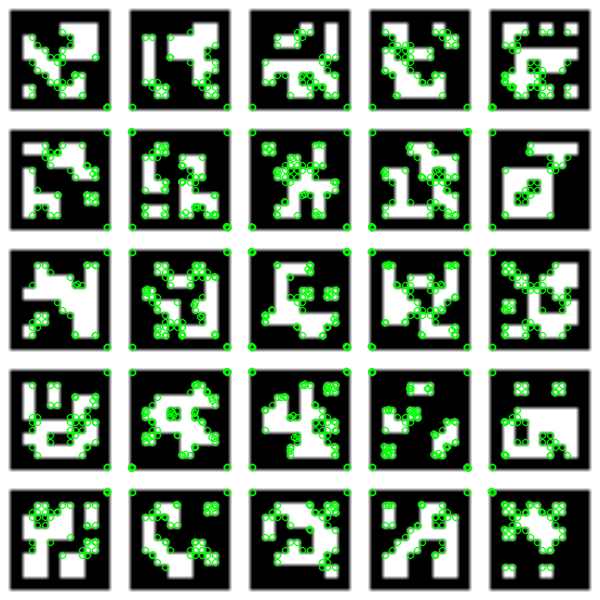
\includegraphics[width=0.45\linewidth]{images/kp_aruco_000.png}
  }
  \hfill
  \subfloat[ArUco\_001 with keypoints \label{AR-KP-02}]{
  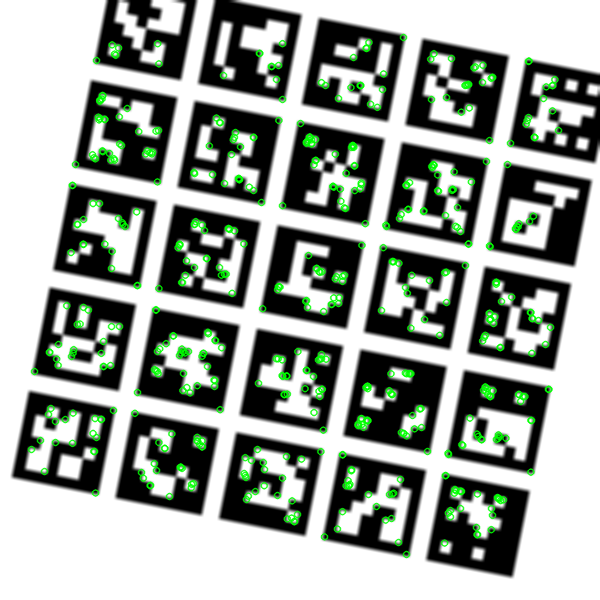
\includegraphics[width=0.45\linewidth]{images/kp_aruco_001.png}
  }
  \caption{Generated images of the keypoint detection test with mapped keypoints}
  \label{fig-KP-AR}
\end{figure}
\end{enumerate}

\paragraph{Feature Description}
\begin{enumerate}
\item \hypertarget{STFR-FD-01}{\textbf{STFR-FD-01}\\}
This test evaluates the capacity of the system to create oriented-BRIEF descriptors using identified keypoints from smoothed greyscale imagery. A target of 100 was set with a search patch size of 31. This test was manually initiated and executed via Pytest using the \href{https://github.com/KiranSingh15/CAS-741-Image-Correspondences/blob/main/src/tests/test_STFR-FD-01.py}{test\_STFR-FD-01.py} program. The test successfully passed all checks and provides a \href{https://github.com/KiranSingh15/CAS-741-Image-Correspondences/blob/main/src/tests/Outputs/2025-04-13_12-17-18/summary.txt}{summary.txt} of the results under its timestamped \href{https://github.com/KiranSingh15/CAS-741-Image-Correspondences/tree/main/src/tests/Outputs/2025-04-13_12-17-18}{STFR-FD-01} output folder. \\ \\
\textit{Requirements Addressed:} 
\begin{itemize}
\item R3 (Update Patch Size)
\item R4 (Update Descriptor Bin Size)
\item R7 (Binary Descriptors)
\item R11 (Define Descriptors)
\end{itemize}

Figure \ref{fig-FD-AR} shows an example of two ArUco markers with keypoints scaled per their feature descriptors. All generated output imagery and corresponding CSV files can be reviewed in the \href{https://github.com/KiranSingh15/CAS-741-Image-Correspondences/tree/main/src/tests/Outputs/2025-04-13_12-17-18}{STFR-FD-01} output folder.\\


\begin{figure}[h!]
  \centering
  \subfloat[ArUco\_000 with scaled keypoints \label{AR-FD-01}]{
  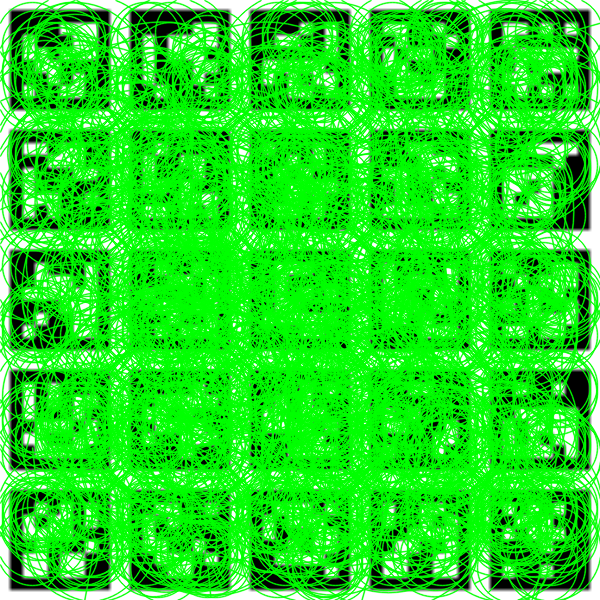
\includegraphics[width=0.45\linewidth]{images/fd_aruco_000.png}
  }
  \hfill
  \subfloat[ArUco\_001 with scaled keypoints \label{AR-FD-02}]{
  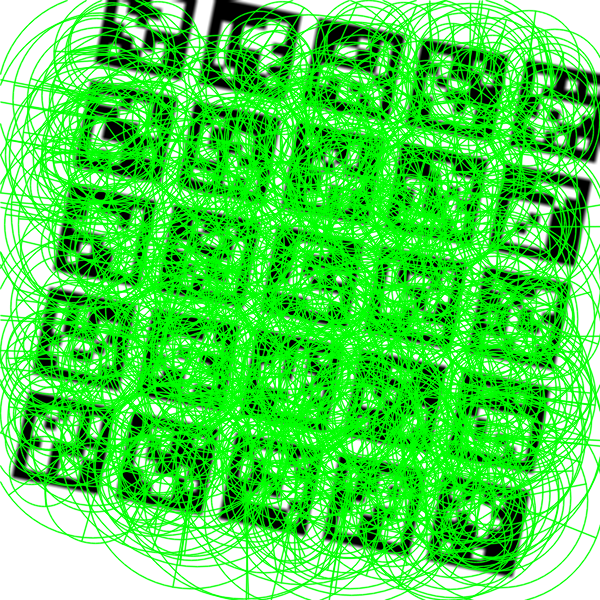
\includegraphics[width=0.45\linewidth]{images/fd_aruco_001.png}
  }
  \caption{Generated images of the keypoint detection test with mapped keypoints}
  \label{fig-FD-AR}
\end{figure}
\end{enumerate}




\subsection{Feature Comparison}
\paragraph{Descriptor Comparison} 

\begin{enumerate}


\item \hypertarget{STFR-FM-01}{\textbf{STFR-FM-01}}\\
This test evaluates the capacity of the system to compare two sets of predefined feature descriptor between two similar images. Using brute-force matching, a maximum Hamming distance of 25 was set for displayed images. Additionally, a maximum of 30 match candidates were permitted to be displayed in the generated imagery. This test was manually initiated and executed via Pytest using the \href{https://github.com/KiranSingh15/CAS-741-Image-Correspondences/blob/main/src/tests/test_STFR-FM-01.py}{test\_STFR-FM-01.py} program. The test successfully passed all checks and provides a \href{https://github.com/KiranSingh15/CAS-741-Image-Correspondences/blob/main/src/tests/Outputs/2025-04-13_12-18-08/summary.txt}{summary.txt} of the results under its timestamped \href{https://github.com/KiranSingh15/CAS-741-Image-Correspondences/tree/main/src/tests/Outputs/2025-04-13_12-18-08}{STFR-FM-01} output folder. \\ \\
\textit{Requirements Addressed:} 
\begin{itemize}
\item R8 (Descriptor Comparison - Hamming Distance)
\item R12 (Search for Matches Candidates)
\item R13 (Verify Match Candidates)
\item R14 (Confirm Pose Identifiers)
\item R15 (Report Match Candidates)
\end{itemize}

Figure \ref{fig-FM-AR} shows an example of thirty candidate feature matches between markers ArUco\_000 and ArUco\_001. All generated output imagery and corresponding CSV files can be reviewed in the \href{https://github.com/KiranSingh15/CAS-741-Image-Correspondences/tree/main/src/tests/Outputs/2025-04-13_12-18-08}{STFR-FM-01} output folder.\\

\begin{figure}
  \centering
  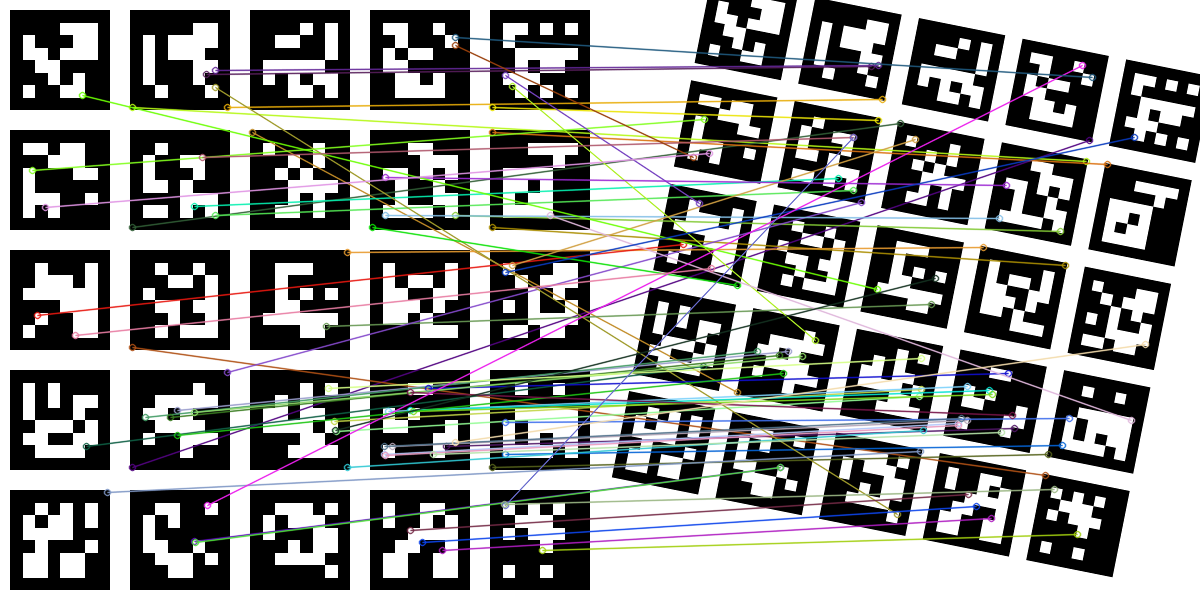
\includegraphics[width=0.95\linewidth]{images/aruco_000_aruco_001.png}
  \caption{Optimal candidate matches between ArUco\_000 and ArUco\_001}
  \label{fig-FM-AR}
\end{figure}



\end{enumerate}



\section{Nonfunctional Requirements Evaluation}
\subsection{Reliability}
\begin{itemize}
  \item NFR1 (Invariance to the Order of Images)
  \end{itemize}
A test script named \href{https://github.com/KiranSingh15/CAS-741-Image-Correspondences/blob/main/src/tests/test_STNFR-RE-01.py}{\textbf{test\_STNFR-RE-01.py}} was prepared. In this script, two images from the \href{https://github.com/KiranSingh15/CAS-741-Image-Correspondences/tree/main/src/tests/testImages/lego}{\textbf{Lego}} image set are renamed and reordered, as outlined in the \href{https://github.com/KiranSingh15/CAS-741-Image-Correspondences/tree/main/src/tests/testImages/lego_swap}{\textbf{Lego\_Swap}} folder. Both of these datasets are processed to identify candidate matches. The resulting match candidates are compared between each data set to confirm that each descriptor and corresponding coordinates from the Lego dataset is matched to the equivalent descriptor in the transformed Lego\_Swap dataset. This test passed with zero errors, and the results are summarized in the \href{https://github.com/KiranSingh15/CAS-741-Image-Correspondences/tree/main/src/tests/Outputs/2025-04-13_15-19-26}{\textbf{STNFR-RE-01}}.


\subsection{Usability}
\textbf{IFCS\_DEMO-01}\\
\begin{itemize}
  \item NFR2 (Simple to Use)
  \end{itemize}
Ten (10) individuals were given a demonstration of the IFCS software, which included a detailed walkthough of the download process, installation processes, and setup of the virtual environment. Audience members were shown how to add new images from the provided library to the inputs folder, adjust the methods and parameters of image processing, and initiate the IFCS pipeline. Once completed, audience members were shown the following outputs.
\begin{itemize}
  \item generated greyscale imagery
  \item generated smoothed imagery
  \item generated imagery with keypoints
  \item generated imagery with descriptors
  \item generated imagery that compare images with candidate descriptor matches
  \item CSV files of keypoints, descriptors and candidate matches
\end{itemize}
Following the demonstration, a show-of-hands identified that seven (7) of ten audience members stated that they have a favourable opinion of the software and its simplicity of use. At a success rate of 70\%, this fall below the target rate of 80\%. However, this may be improved with the implementation of any one of a user manual, user walkthrough video, or a one-on-one training session with one of the IFCS developers.

\subsection{Maintainability}
\textit{Requirements Addressed:} 
\begin{itemize}
\item NFR3 (Allocation of Developer Resources for New Features)
\end{itemize}
Per the \href{https://github.com/KiranSingh15/CAS-741-Image-Correspondences/blob/main/docs/VnVPlan/VnVPlan.pdf}{\textbf{VnV Plan}}, this requirement has been identified as out of scope for the Rev 1.0 release.
		
\subsection{Performance}
\textit{Requirements Addressed:} 
\begin{itemize}
\item NFR4 (Timing Metrics)
\item NFR5 (Memory Usage Metrics)
\end{itemize}
Timing metrics and memory usage were identified as test features of interest for the lifespan of the IFCS software. These tools would be appended to compare the relative performance of different methods such as FAST and Harris scores for keypoint detection. However, as the scope of the Winter 2025 development cycle narrowed to prioritize robust performance of ORB feature detection and brute-force matching, the implementation of timing metrics will be deferred to the development cycle of Summer 2025. These metric wil be assessed as part of the systems tests as follows through the \href{https://pypi.org/project/pytest-monitor/}{Pytest Monitor} plugin, which has the capacity to assess both timing and memory metrics and is suitable for integration with GitHub Actions.

	
\section{Comparison to Existing Implementation}	
This section is \textbf{not applicable}.

\section{Unit Testing}
All unit tests are automated to run via a pull request and Pytest Github Actions. These tests can be found in the \href{https://github.com/KiranSingh15/CAS-741-Image-Correspondences/tree/main/test}{\textbf{test}}. Each test is initiated by the \href{https://github.com/KiranSingh15/CAS-741-Image-Correspondences/blob/main/test/run_unit_checks.py}{\textbf{run\_unit\_checks.py}} program, as shown in Figure \ref{unit_tests}. Upon completion of the unit tests a \href{https://github.com/KiranSingh15/CAS-741-Image-Correspondences/blob/main/test/results/UnitTests-60f8e10/2025-04-15_01-38-43/summary.txt}{\textbf{summary}} file is generated that outlines the quantity of tests that have passed or failed for each module, as shown in Figure \ref{unit_tests_summary}. In the same folder, a detailed summary of all unit tests for each module is outlined, as shown in Figure \ref{unit_tests_reports}. A detailed example of the unit test report for the \textbf{Specification Parameters Module (M4)} is outlined in Figure \ref{sp_report}. All unit tests were shown to have passed successfully for each module.

\begin{figure}[h!]
  \centering
  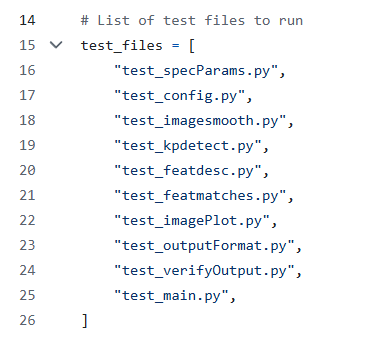
\includegraphics[width=0.65\linewidth]{images/unit_test_names.png}
  \caption{Outline of automated unit tests}
  \label{unit_tests}
\end{figure}

\begin{figure}[h!]
  \centering
  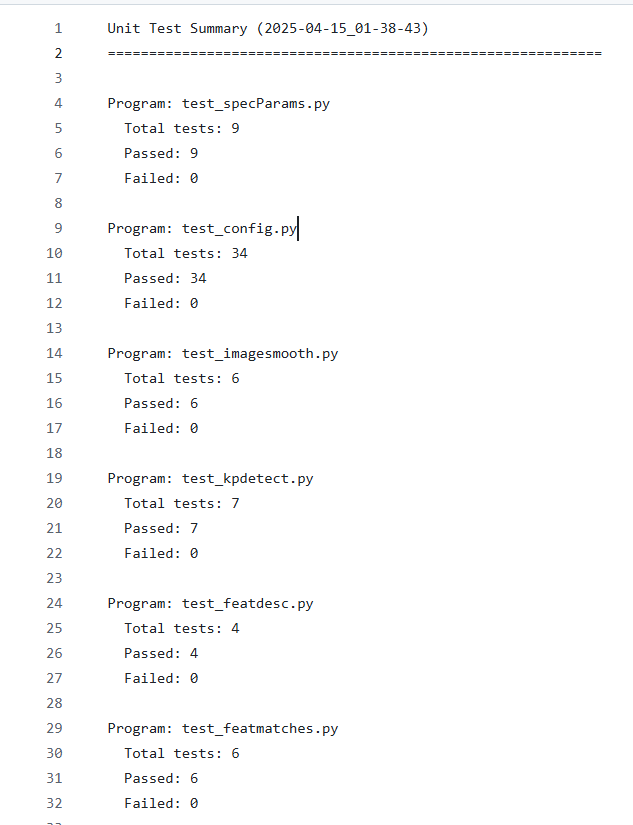
\includegraphics[width=0.8\linewidth]{images/ut_pass_fail.png}
  \caption{Unit Test Summary.txt}
  \label{unit_tests_summary}
\end{figure}

\begin{figure}
  \centering
  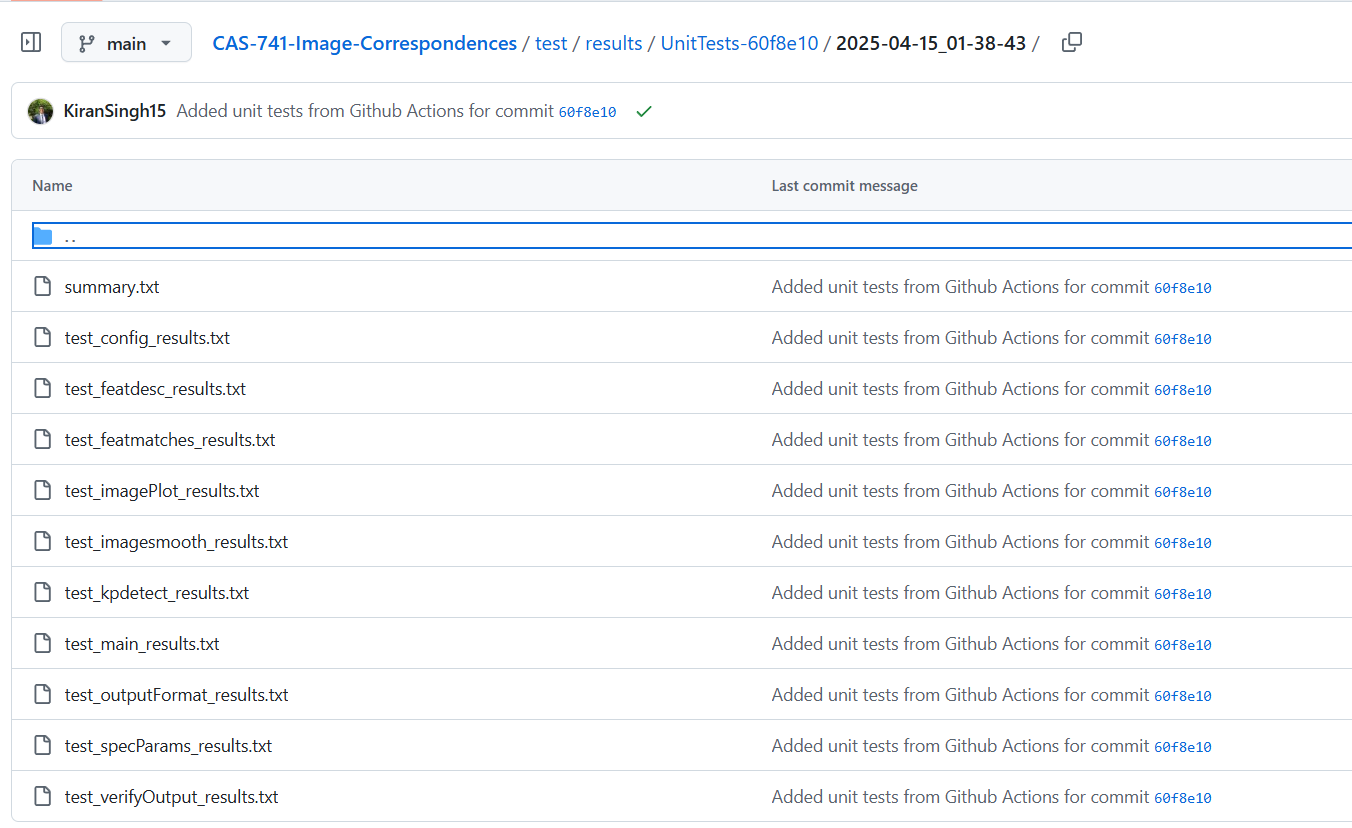
\includegraphics[width=1.2\linewidth]{images/ut_reports.png}
  \caption{Generated Unit Test Reports}
  \label{unit_tests_reports}
\end{figure}

\begin{figure}
  \centering
  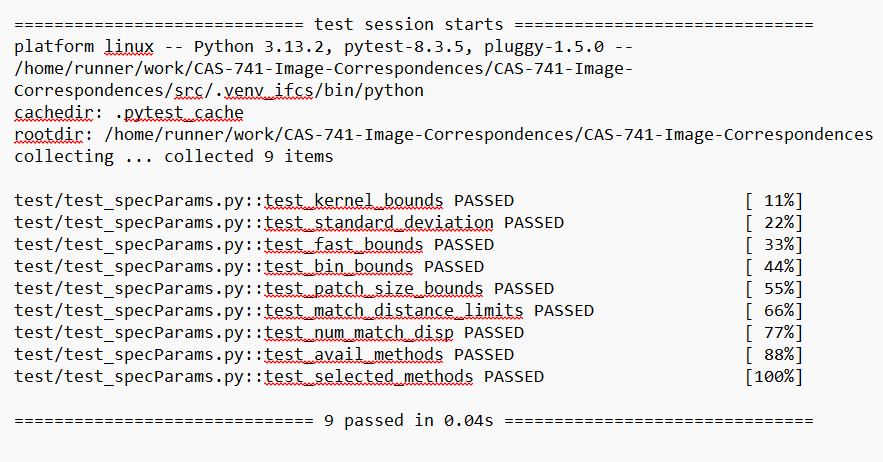
\includegraphics[width=0.9\linewidth]{images/specParams_report.png}
  \caption{Specification Parameters Unit Test Report}
  \label{sp_report}
\end{figure}


\section{Changes Due to Testing}

This section summarizes the most significant changes made to the modules and test infrastructure as a result of iterative testing, user feedback, and supervisor reviews, particularly following the Rev 0 demonstration. Each change was implemented to improve traceability, robustness, or test validation.

\begin{enumerate}
  \item \textbf{Unification of Output Directory Structure} \\
  All outputs from functional tests (grayscale, smoothed images, keypoints, descriptors, and matches) are now saved under a single, timestamped path: \texttt{tests/Outputs/<timestamp>/}. This change was made in response to confusion around inconsistent file locations during test runs. It ensures better organization, test reproducibility, and avoids polluting production outputs.

  \item \textbf{Validation of CSV Content and Structure} \\
  Functional tests now verify not only the existence of output files but also the correctness of their internal structure, including column names and row counts. For example, descriptor CSVs must contain binary string columns, and match files must include both descriptors and matching scores. This change prevents false positives where tests previously passed despite incomplete or invalid outputs.

  \item \textbf{Enforcement of Parameter Bounds} \\
  Dedicated unit tests were introduced to ensure that all configurable parameters (e.g., Gaussian kernel size, standard deviation, patch size, bin count, match threshold) are within valid numerical and type constraints. These checks catch invalid user input early, reducing undefined behavior during runtime.

  \item \textbf{Synthetic Imagery for CI Integration} \\
  A minimal testing pipeline using synthetic image pairs was implemented in \texttt{test\_main.py}. This allows the pipeline to be tested in continuous integration (CI) environments without relying on external image datasets. It also ensures the processing pipeline can execute end-to-end with minimal dependencies.

  \item \textbf{Inclusion of Feature Metadata in Match Results} \\
  Feature match outputs were extended to include 256-bit binary descriptors for both the query and train features, image IDs, and matching scores. This change enables deeper validation of match quality and allows visual or statistical analysis of correspondence accuracy in test reports.

  \item \textbf{Standardized Test Summaries for Reporting} \\
  Each test script now generates a summary file (e.g., \texttt{test\_kpdetect\_results.txt}, \texttt{test\_main\_results.txt}) detailing test names, pass/fail status, and parameters. This facilitates automated result aggregation in CI pipelines and provides a consistent audit trail for testing history.
\end{enumerate}


\section{Automated Testing}
All unit tests are automated to run via a pull request and Pytest Github Actions. These tests can be found in the \href{https://github.com/KiranSingh15/CAS-741-Image-Correspondences/tree/main/test}{\textbf{test}}. Each test is initiated by the \href{https://github.com/KiranSingh15/CAS-741-Image-Correspondences/blob/main/test/run_unit_checks.py}{\textbf{run\_unit\_checks.py}} program, as shown in Figure \ref{unit_tests}. 

		
\section{Trace to Requirements}
The traceability of both functional and nonfunctional requirements to system tests can be found in Table \ref{Requirements_SystemTests}. We note that the functional requirements are entirely covered by the outlined tests. We also note that NFR3 has been omitted from the scope of testing, and that NF4 and NFR5 has been deferred at the time of release for Rev 1.0 due to resource constraints within the development team. Testing for these requirements will be implemented as part of development during the Summer of 2025.

\begin{table}[h!]
  \centering
  \renewcommand{\arraystretch}{1.4}
  \resizebox{1.2\textwidth}{!}{%
  \begin{tabular}{|c|c|c|c|c|c|l|}
  \hline
  \textbf{Requirement} & \textbf{STFR-IS-01} & \textbf{STFR-KP-01} & \textbf{STFR-FD-01} & \textbf{STFR-FM-01} & \textbf{STNFR-RE-01} & \multicolumn{1}{c|}{\textbf{IFCS-DEMO-01}} \\ \hline
  R1 & X &  &  &  &  &  \\ \hline
  R2 &  & X &  &  &  &  \\ \hline
  R3 &  &  & X &  &  &  \\ \hline
  R4 &  &  & X &  &  &  \\ \hline
  R5 & X &  &  &  &  &  \\ \hline
  R6 &  & X &  &  &  &  \\ \hline
  R7 &  &  & X &  &  &  \\ \hline
  R8 &  &  &  & X &  &  \\ \hline
  R9 & X &  &  &  &  &  \\ \hline
  R10 &  & X &  &  &  &  \\ \hline
  R11 &  &  & X &  &  &  \\ \hline
  R12 &  &  &  & X &  &  \\ \hline
  R13 &  &  &  & X &  &  \\ \hline
  R14 &  &  &  & X &  &  \\ \hline
  R15 &  &  &  & X &  & \multicolumn{1}{c|}{} \\ \hline
  NFR1 &  &  &  &  & X &  \\ \hline
  NFR2 &  &  &  &  &  & \multicolumn{1}{c|}{X} \\ \hline
  NFR3 & - & - & - & - & - & \multicolumn{1}{c|}{-} \\ \hline
  NFR4* & - & - & - & - & - & \multicolumn{1}{c|}{-} \\ \hline
  NFR5* & - & - & - & - & - & \multicolumn{1}{c|}{-} \\ \hline
  \end{tabular}
  }
  \caption{Traceability matrix between modules and identified unit tests}
  \label{Requirements_SystemTests}
  \end{table}




\section{Trace to Modules}		
A full outline of the traceability between the unit tests and the modules as outlined in the MIS is provided in Table \ref{tab:mod_units}.

% Define plain text symbols
\newcommand{\markinit}{\texttt{/}}   % initialization
\newcommand{\markyes}{\texttt{x}}    % module tested
\newcommand{\markna}{\texttt{-}}     % not applicable

\begin{table}[htbp]
  \centering
  \renewcommand{\arraystretch}{1.4}
  \resizebox{1.2\textwidth}{!}{%
  \begin{tabular}{|l|c|c|c|c|c|c|c|c|c|c|c|}
  \hline
  \textbf{Test Name} & \textbf{M1} & \textbf{M2} & \textbf{M3} & \textbf{M4} & \textbf{M5} & \textbf{M6} & \textbf{M7} & \textbf{M8} & \textbf{M9} & \textbf{M10} & \textbf{M11} \\
  \hline
  test\_pipeline\_synthetic\_images & \markinit & \markyes & \markna & \markna & \markna & \markna & \markna & \markna & \markna & \markna & \markna \\
  \hline 
  test\_check\_parameter\_limits\_valid & \markinit & \markna & \markyes & \markna & \markna & \markna & \markna & \markna & \markna & \markna & \markna \\
  test\_check\_method\_limits\_valid & \markinit & \markna & \markyes & \markna & \markna & \markna & \markna & \markna & \markna & \markna & \markna \\
  test\_check\_method\_limits\_invalid & \markinit & \markna & \markyes & \markna & \markna & \markna & \markna & \markna & \markna & \markna & \markna \\
  \hline

  test\_kernel\_bounds & \markinit & \markna & \markna & \markyes & \markna & \markna & \markna & \markna & \markna & \markna & \markna \\
  test\_standard\_deviation & \markinit & \markna & \markna & \markyes & \markna & \markna & \markna & \markna & \markna & \markna & \markna \\
  test\_fast\_bounds & \markinit & \markna & \markna & \markyes & \markna & \markna & \markna & \markna & \markna & \markna & \markna \\
  test\_bin\_bounds & \markinit & \markna & \markna & \markyes & \markna & \markna & \markna & \markna & \markna & \markna & \markna \\
  test\_patch\_size\_bounds & \markinit & \markna & \markna & \markyes & \markna & \markna & \markna & \markna & \markna & \markna & \markna \\
  test\_avail\_methods & \markinit & \markna & \markna & \markyes & \markna & \markna & \markna & \markna & \markna & \markna & \markna \\
  test\_selected\_methods & \markinit & \markna & \markna & \markyes & \markna & \markna & \markna & \markna & \markna & \markna & \markna \\
  \hline
  
  test\_output\_keypoints\_variable\_size & \markinit & \markna & \markna & \markna & \markyes & \markna & \markna & \markna & \markna & \markna & \markna \\
  test\_output\_descriptors\_variable\_size & \markinit & \markna & \markna & \markna & \markyes & \markna & \markna & \markna & \markna & \markna & \markna \\
  test\_output\_matches\_variable\_size & \markinit & \markna & \markna & \markna & \markyes & \markna & \markna & \markna & \markna & \markna & \markna \\
  \hline

  test\_check\_match\_uniqueness\_valid & \markinit & \markna & \markna & \markna & \markna & \markyes & \markna & \markna & \markna & \markna & \markna \\
  test\_check\_match\_uniqueness\_warns\_for\_same\_ids & \markinit & \markna & \markna & \markna & \markna & \markyes & \markna & \markna & \markna & \markna & \markna \\
  test\_check\_match\_uniqueness\_warns\_with\_matches & \markinit & \markna & \markna & \markna & \markna & \markyes & \markna & \markna & \markna & \markna & \markna \\
  \hline

  test\_smooth\_image\_valid\_gaussian & \markinit & \markna & \markna & \markna & \markna & \markna & \markyes & \markna & \markna & \markna & \markna \\
  \hline

  test\_detect\_keypoints\_with\_valid\_orb & \markinit & \markna & \markna & \markna & \markna & \markna & \markna & \markyes & \markna & \markna & \markna \\
  \hline

  test\_compute\_descriptors\_valid & \markinit & \markna & \markna & \markna & \markna & \markna & \markna & \markna & \markyes & \markna & \markna \\
  \hline

  test\_match\_features\_no\_loss & \markinit & \markna & \markna & \markna & \markna & \markna & \markna & \markna & \markna & \markyes & \markna \\
  \hline

  test\_gen\_kp\_img\_with\_none\_keypoints & \markinit & \markna & \markna & \markna & \markna & \markna & \markna & \markna & \markna & \markna & \markyes \\
  test\_gen\_kp\_img\_no\_flag & \markinit & \markna & \markna & \markna & \markna & \markna & \markna & \markna & \markna & \markna & \markyes \\
  test\_gen\_kp\_img\_rich\_keypoints & \markinit & \markna & \markna & \markna & \markna & \markna & \markna & \markna & \markna & \markna & \markyes \\
  test\_gen\_kp\_img\_with\_none\_image & \markinit & \markna & \markna & \markna & \markna & \markna & \markna & \markna & \markna & \markna & \markyes \\
  test\_gen\_matched\_features\_success & \markinit & \markna & \markna & \markna & \markna & \markna & \markna & \markna & \markna & \markna & \markyes \\



  \hline
  \end{tabular}%
  }
  \caption{Traceability matrix mapping unit tests to associated software modules(M2–M11).}
  \label{tab:mod_units}
  \end{table}
\section{Code Coverage Metrics}

\bibliographystyle{plainnat}
\bibliography{../../refs/References}

\end{document}